
What follows are instructions for interacting with the Galant GUI interface.

\subsection{Overview}

Galant provides three major components across two windows:
\begin{enumerate}
\item
a text window that can serve two distinct purposes --
\begin{enumerate}
\item as an editor of algorithms
\item as an editor of GraphML representations of graphs
\end{enumerate}
\item
a graph window that displays the current graph (independent of whether
the text window shows an algorithm or the GraphML representation of the graph)
\end{enumerate}

It should be noted that it is usually more convenient to edit algorithms
offline using a program editor and to use the visual editor only to edit graphs
-- one exception is when a precise lining up of node positions is desired.

\begin{figure}[p!]
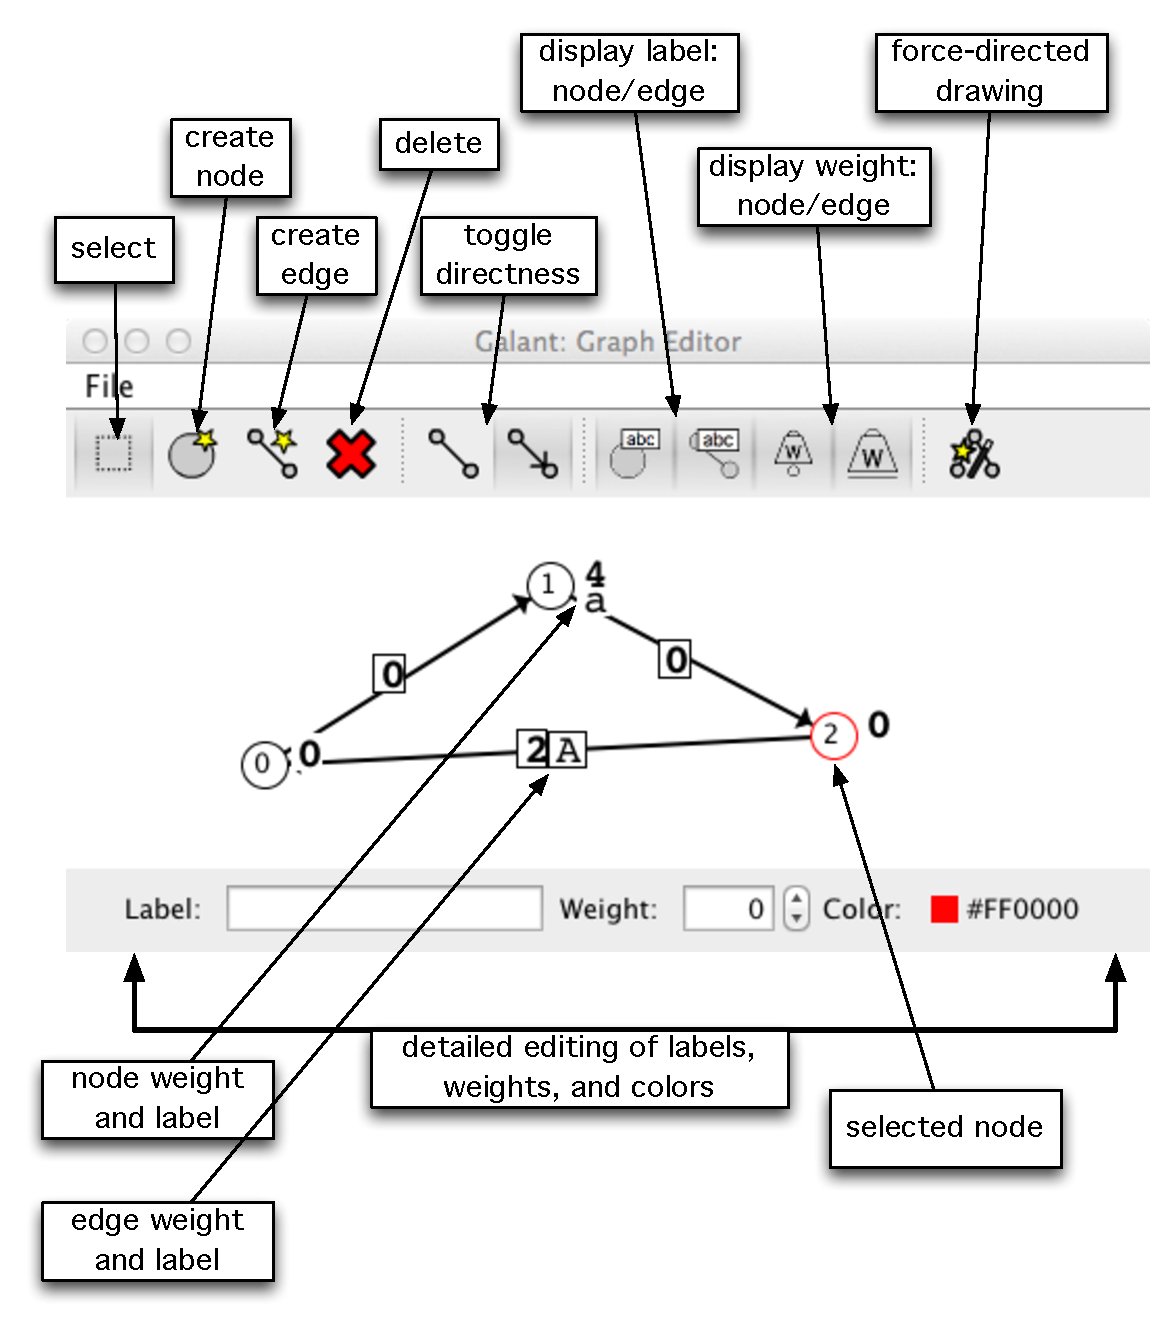
\includegraphics[scale=0.5]{X_graph_window_annotated}
\caption{The Galant graph window with annotations.}
\label{fig:graph_window_annotated}
\end{figure}

\begin{figure}[p!]
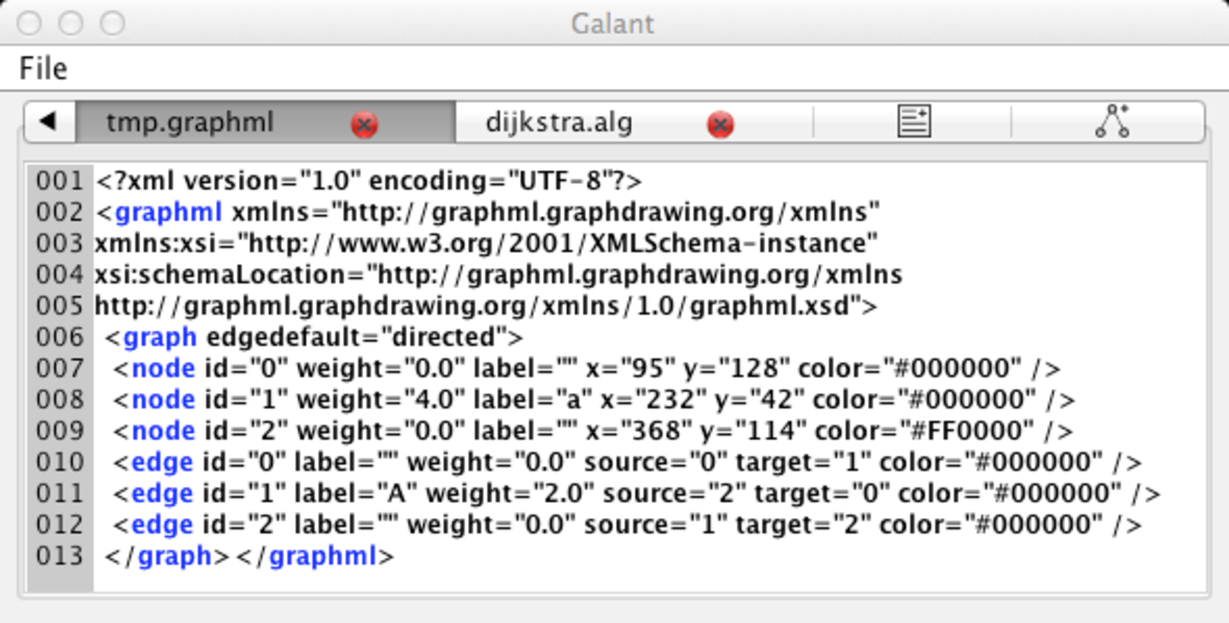
\includegraphics[scale=0.5]{X_graphml_window}
\caption{The text window with the GraphML representation of the graph in
Fig.~\ref{fig:graph_window_annotated}.}
\label{fig:graphml_window}
\end{figure}

\begin{figure}[p!]
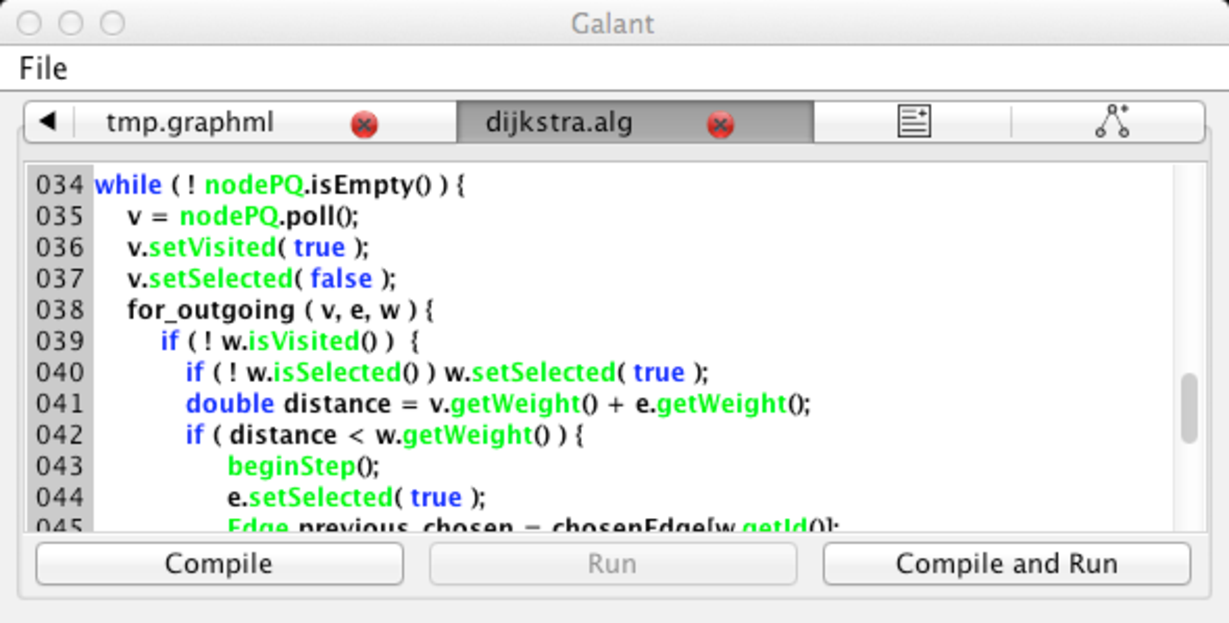
\includegraphics[scale=0.5]{X_algorithm_window}
\caption{The text window showing Dijkstra's algorithm.}
\label{fig:algorithm_text}
\end{figure}

\begin{figure}[p!]
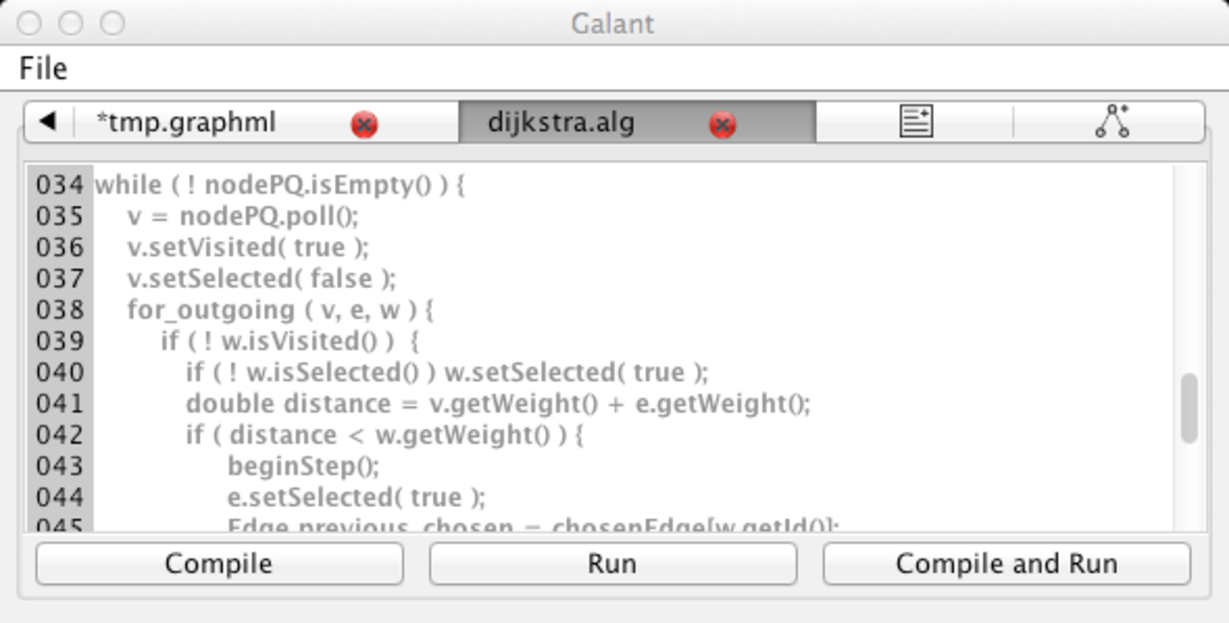
\includegraphics[scale=0.5]{X_algorithm_running}
\caption{The text window when Dijkstra's algorithm is running.}
\label{fig:algorithm_running}
\end{figure}

\begin{figure}[p!]
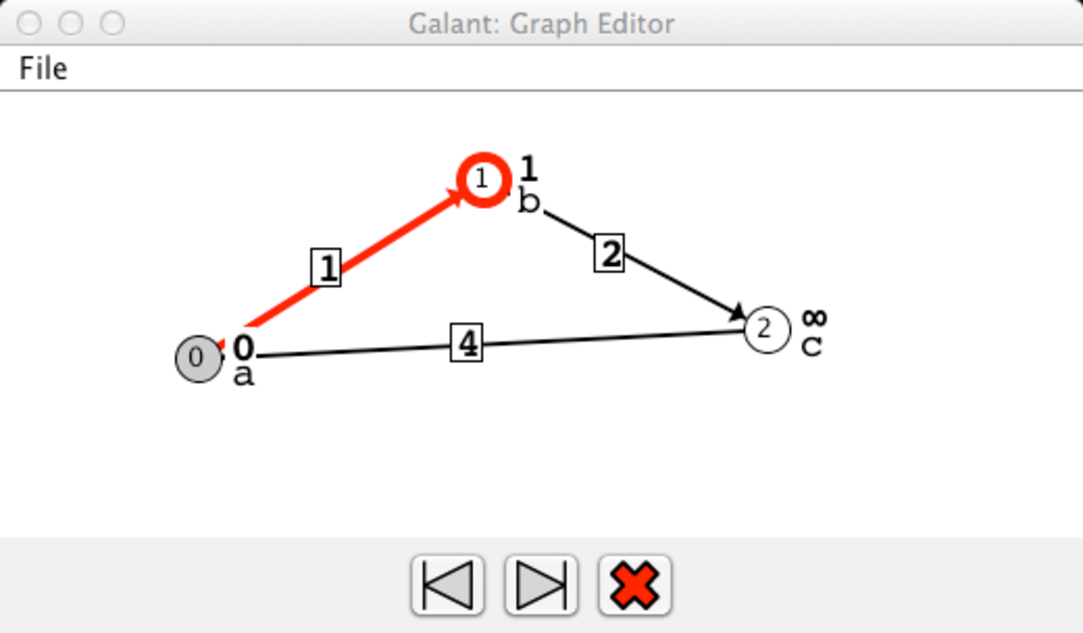
\includegraphics[scale=0.5]{X_dijkstra_running}
\caption{The graph window when Dijkstra's algorithm is running.}
\label{fig:dijkstra_running}
\end{figure}

These components operate in two modes: edit mode and animation mode.
Edit mode allows the user to modify graphs -- see Sec.~\ref{sec:graph_editing},
or algorithms -- see Sec.~\ref{sec:algorithm_editing}. Animation mode disables all forms of modification, allowing the user to progress through
an animation by stepping forward or backward, as described in
Sec.~\ref{sec:animating_algorithms}.

\subsection{Workspace}

Opened graph and algorithm files are displayed in the text window,
which has tabs that allow the user to switch among different algorithms/graphs.
New algorithms can be created using the ``page'' icon at the top right of the
window and new graphs using the graph/tree icon to the left of that.
More commonly, algorithm and graph files are loaded via the \texttt{File->Open}
browser dialog. The \texttt{File} drop-down menu also allows saving of files
and editing preferences. Algorithm files have the extension \texttt{.alg}
and graph files the extension \texttt{.graphml}.

\subsection{Graph editing}
\label{sec:graph_editing}

Graphs can be edited in their GraphML representation using the text window
or visually using the graph window.
These editors are linked:
any change in the visual representation is immediately reflected in the text
representation (and will overwrite what was originally there);
a change in the GraphML representation will take effect in the visual representation
when the file is saved.

An improperly formatted GraphML file loaded form an external source will
show as blank in the text window -- unfortunately there is no error
reporting in the current Galant implementation.
The graph window, as illustrated in Fig.~\ref{fig:graph_window_annotated}
has a toolbar with four sections:
\begin{enumerate}
\item
\textbf{Graph edit mode -- }
this includes the \emph{select}, \emph{create node}, \emph{create edge}, and \emph{delete} buttons.
Only one button is active at any time; it determines the effect
of a user's interaction (mouse clicking, dragging, etc.) with the window.
if there are conflicts in selection of objects, nodes with higher id numbers have precedence (are above those with lower id numbers) and nodes
have precedence over edges (are above edges).
\begin{itemize}
\item \emph{Select.} A mouse click selects the graph component with highest precedence.
If the component is a node, it is shaded; if it's an edge, it turns blue.
The inline editor at the bottom of the graph window allows editing of the
component's label, weight, and color.
\item \emph{Create node.}
A node is created at the location of a mouse click if there is not already a node there.
If another node is present it is simply selected.
\item \emph{Create edge.}
Two clicks are required to create an edge. The first falls on the desired
source node and the second on the destination node.
The line representing the edge is shown after the first click.
If the first click does not land on a node, no edge is created.
If the second click does not land on a node, creation of the edge is canceled.
\item \emph{Delete.}
A mouse click deletes the highest-precedence component at the mouse location.
If a node is deleted, all of its incident edges are deleted as well.
\end{itemize}

\item
\textbf{Directedness toggles --}
These change both the interpretation and the
display of the graph between directed and undirected.
Pressing the undirected (line between two dots) button causes
all edges to be interpreted as undirected: this means that, when the code
calls for all incoming/outgoing edges, all incident edges are used.
Undirected edges are displayed as simple lines.

Pressing the directed (line with arrow) button causes the macros
\texttt{for\_incoming}, \texttt{for\_outgoing}, and \texttt{for\_adjacent}
to have three distinct meanings (they are all the same for undirected graphs):
Incoming edges have the given node as destination, outgoing as source, and adjacent applies to all incident edges.

\item
\textbf{Display toggles --}
The four display toggles turn on/off the display of node/edge labels and node/edge weights.
A shaded toggle indicates that the corresponding display is \emph{on}.
When Galant is executed for the first time, all of these are \emph{on},
but their setting persists from session to session.

\item
\textbf{Force directed drawing button -- }
Applies Hu's force directed algorithm~\cite{2006-Mathematica-Hu} to the graph.
\emph{Caution: this operation cannot be undone.}

\end{enumerate}

\subsection{Algorithm editing}
\label{sec:algorithm_editing}

Algorithms can be edited in the text window. The
editor uses Java keyword highlighting (default blue) and
highlighting of Galant API fields and methods (default green).
Since the current algorithm editor is fairly primitive (no search and replace, for example),
it is more efficient to edit animation code offline using a program editor --
for example \texttt{emacs} with Java mode turned on.
The Galant editor is, however, useful for locating and correcting minor errors.
For more details on how to compose animation code, see the programmer guide
(Section~\ref{sec:programmer_guide}).

\subsection{Animating algorithms}
\label{sec:animating_algorithms}

To animate an algorithm the code for it must be compiled and then run via the
algorithm controls
 -- the bottom tabs on the text window shown in Figs.~\ref{fig:algorithm_text}
and~\ref{fig:algorithm_running}.
The algorithm runs on the \emph{active graph}, the one currently displayed
on the graph window.
If there are errors in compilation these will show up on the console (terminal
from which Galant was run) -- this will be fixed in later revisions.
Runtime errors open a dialog box that allows the user to ask for more details
and decide whether to exit Galant or not.

Algorithms are executed to completion. After that the step forward and step
back buttons (arrow buttons at the bottom of the graph window shown in Fig.~\ref{fig:dijkstra_running}) can be used to move forward or backwards through the execution.
The left and right arrow keys on the keyboard have the same effect
\emph{but the graph window must be in focus} (by default the panel
containing the buttons at the
bottom is in focus).
Mixing button presses with keyboard shortcuts is not advisable --
there are currently some bugs that may cause strange behavior if an animation
involves position changes.

During the execution of the animation, all graph editing functions are disabled.
These are re-enabled when the user exits the animation by pressing the red \textbf{X} button.

\subsection{Preferences}
\label{sec:preferences}

Galant preferences can be accessed via the \texttt{File->Preferences}
menu item or by using the keyboard shortcut Ctrl+Shift+P (Cmd+Shift+P for Mac).
Preferences that can be edited are:
\begin{itemize}
\item
Default directories for opening and saving files (\texttt{Open/Save}).
\item
Directory where compiled animation code is stored (\texttt{Compilation}).
\item
Font size and tab size for text window editing (\texttt{Editors}).
\item
Colors for keyword and Galant API highlighting (\texttt{Algorithm~Editor}).
\item
Color for GraphML highlighting (\texttt{Textual~Graph~Editor}).
\item
Edge width (\texttt{Visual~Graph~Editor}).
\end{itemize}


% [Last modified: 2013 06 04 at 19:29:25 GMT]
